\subsection{MNIST}
We compare the the distribution of features computed over the MNIST train data
to the distribution of the same features computed over MNIST test data, samples
generated with LSGAN, improved WGAN, adversarial samples computed using the fast gradient
sign method. The training data is scaled to $[-1, 1]$ and the scaled baseline is sampled from a binomial distribution with number of trials 1
and probability of success equal to the normalized mean value of pixel intentities in the
MNIST training data, 0.13. The discriminator and the generator follow the DCGAN architecture.
The classifier used to generate the adversarial samples is a three layer fully
conected network with dropout on every layer (25\%, 50\%, 50\%) and rectified
linear units on the first and second layers. The $\epsilon$ parameter for the
adversarial attack is set to $.25$(CHECK IF NOT $.1$). 
Following common practice in GAN training, each GAN model is trained until the
loss plateaus and we are satisfied with the quality of the output.  

Figure \ref{fig:mnist_samples} shows samples drawn from MNIST train, test,
LSGAN, IWGAN, FSGM and binomial respectively. 
\begin{figure}[!h]
  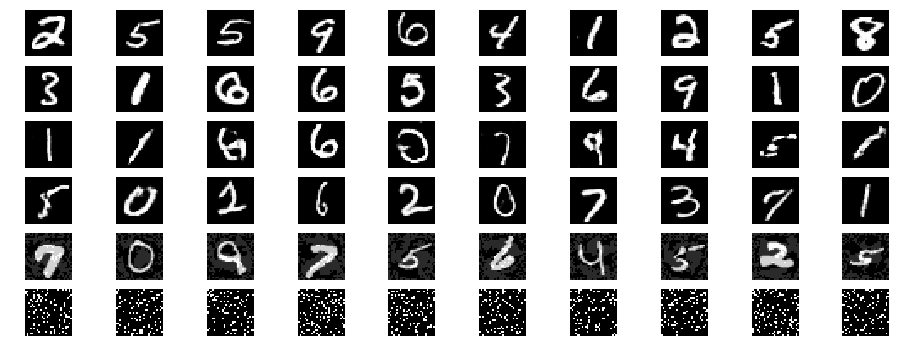
\includegraphics[width=\linewidth]{mnist_samples.png}
  \caption{}
  \label{fig:mnist_samples}
\end{figure}

Visual inspection of these generated samples can lead one to believe that IWGAN
produces better samples than the LSGAN. Below we compare the distribution of
pixel intensities of several data to MNIST's training data. 
Table~\ref{tbl:mnist_pixel} reveals that although the pixel intensities of LSGAN
and IWGAN samples look similar to the training data, they are considerably
different given the KS Two Sample Test\footnote{Remember that the
    test statistic is inversely proportial to $\sqrt{n}$}but not so different given the JSD. This
can phaenomena can be understood by investigation of the empirical CDF of these
samples in Figure~\ref{fig:mnist_pixel_ecdf}. The pixel values of the samples
generated with the GAN framework are mainly bimodal but distributed around $-1$
and $1$.  Such behavior will be present in any gradient descent method using an
asymptotically converging non-linearity, such as sigmoid and tanh, immediately 
preceding the output of the generating function.


\begin{table}[!h]
\centering
\caption{KS Two Sample Test and JSD over the distribution of pixel values for
different samples}
\label{tbl:mnist_pixel}
\begin{tabular}{l|ll|l|}
                   & \multicolumn{2}{c|}{\cellcolor[HTML]{C0C0C0}KS Two Sample Test} & \multicolumn{1}{c|}{\cellcolor[HTML]{C0C0C0}JSD} \\
                   & Statistic   & P-Value        &                \\
mnist\_train       & 0.0         & 1.0            & 0.0            \\
mnist\_test        & 0.003177    & 8.501950e-35   & 2.955323e-05   \\
mnist\_lsgan       & 0.808119    & 0.0            & 0.013517       \\
mnist\_iwgan       & 0.701573    & 0.0            & 0.014662       \\
mnist\_adversarial & 0.419338    & 0.0            & 0.581769       \\
mnist\_binomial    & 0.130855    & 0.0            & 0.0785009      
\end{tabular}
\end{table}


\begin{figure}[!h]
  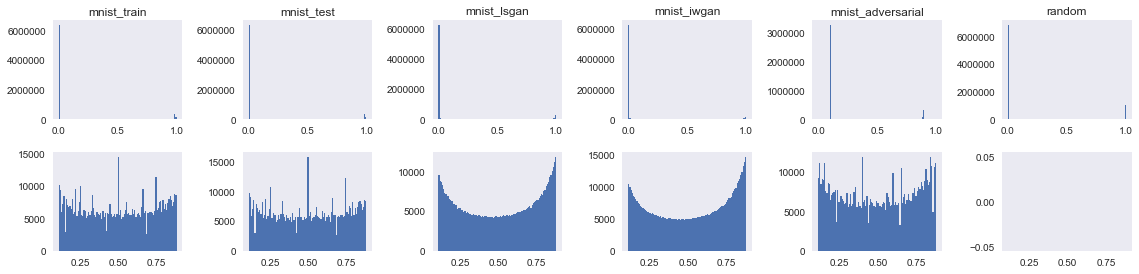
\includegraphics[width=\linewidth]{mnist_pixel_distribution.png}
  \caption{}
  \label{fig:mnist_pixel_distribution}
\end{figure}


\begin{figure}[!h]
  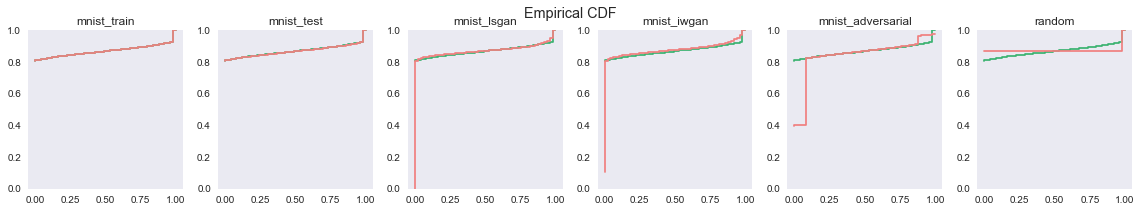
\includegraphics[width=\linewidth]{mnist_pixel_ecdf.png}
  \caption{}
  \label{fig:mnist_pixel_ecdf}
\end{figure}


Although this confirms our hypothesis~\ref{hyp:visual} that there are properties
that are hardly noticed with non-computational inspection, an adversary could
easily apply thresholding to compensate for the asymptotically converging
non-linearity such that the distribution of pixel values of fake
samples become more similar to the real data.

For this reason, we use the distributions over other features on the real and
fake data. Figure~\ref{fig:mnist_slope_distribution} shows
that if on the one hand the distribution of slopes of the test data is similar to the
training data, on the other hand this distribution on generated samples differs
considerably from the training data, thus confirming hypothesis~\ref{hyp:difference}.
In table~\ref{tbl:mnist_slope} we show results of test statistics.

\begin{table}[!h]
\centering
\caption{KS Two Sample Test and JSD over the distribution of mean slope for
different samples}
\label{tbl:mnist_slope}
\begin{tabular}{l|ll|l|}
                   & \multicolumn{2}{c|}{\cellcolor[HTML]{C0C0C0}KS Two Sample Test} & \multicolumn{1}{c|}{\cellcolor[HTML]{C0C0C0}JSD} \\
                   & Statistic   & P-Value    &            \\
mnist\_train       & 0.0         & 1.0        & 0.0        \\
mnist\_test        & 0.030699    & 0.000156   & 0.001872   \\
mnist\_lsgan       & 0.317200    & 0.0        & 0.177692   \\
mnist\_iwgan       & 0.478300    & 0.0        & 0.232894   \\
mnist\_adversarial & 0.309099    & 0.0        & 0.022110   \\
mnist\_binomial    & 0.293200    & 0.0        & 0.084448   
\end{tabular}
\end{table}

\begin{figure}
  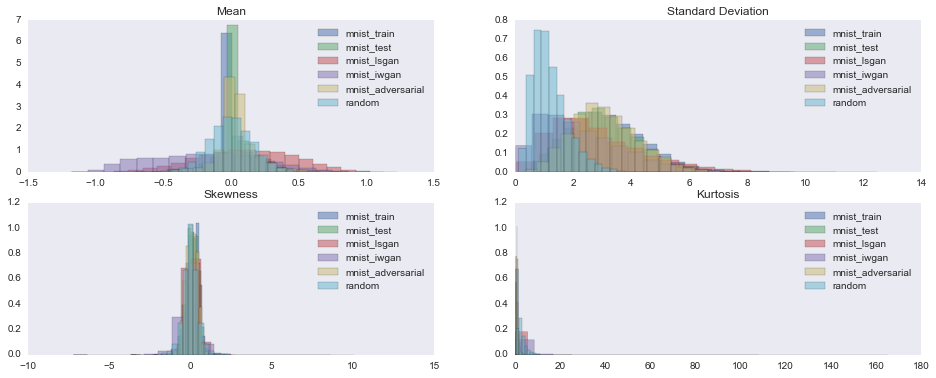
\includegraphics[width=\linewidth]{mnist_slope_distribution.png}
  \caption{}
  \label{fig:mnist_slope_distribution}
\end{figure}

\subsection{Bach Chorales}
\subsection{Speech}
